% set the document type and the font size
\documentclass[spanish, 12pt]{article}

% use Spanish package
\usepackage[spanish]{babel}

% captions without name
\usepackage{caption}

% insert images
\usepackage{graphicx}
\graphicspath{ {img/} }

% set UTF-8 codification
\usepackage[utf8]{inputenc}

% set contents to page using [H]
\usepackage{float}

% insert graphical tree
\usepackage{tikz}
\usepackage{tikz-qtree}

% no equation numeration
\usepackage{amsmath}

% graphs with arrows
\usepackage[all]{xy}

% centering xy graphs
\usepackage{calc}

% cool boxes
\usepackage{fancybox}

\title{Sistemas Operativos}
\author{Diego Enrique Fontán, CosasDePuma}
\date{2017-18}


\begin{document}

	\pagenumbering{gobble}
	\maketitle
	\newpage
	
	\tableofcontents
	\newpage
	
	\pagenumbering{arabic}
	
	\section{Niveles de software}
	
	\vfill
	
		Se denomina \textbf{soporte lógico} o \textbf{software} a todo aquel conjunto de programas asociados a un ordenador.\\
		
		\begin{figure}[H]
			\centering
			\Tree [.Software Aplicaciones Utilidades Control ]
			\caption*{\textit{Niveles de software}}
		\end{figure}
		
		\subsection{Concepto de Sistema Operativo}
		
			Un \textbf{Sistema Operativo} es un programa (o conjunto de subprogramas o módulos) de \underline{control} que tiene como finalidad facilitar el uso del ordenador y conseguir que se utilice eficientemente.\\
			
			\subsubsection{Características del Sistema Operativo}
			
				- Actúa como interfaz entre el usuario y la máquina física.\\
			
				- Controla la ejecución de otros programas.\\
				
				- Gestiona y mantiene ficheros.\\
			
				- Contabiliza la utilización de los recursos.\\
			
				- Protege los datos y los programas.\\
			
				- Gestiona y asigna directamente los recursos hardware.
				
				\begin{equation}
					\notag
					\vdots
				\end{equation}
				
				\newpage
		
			\subsubsection{Funciones principales del Sistema Operativo}
		
				El Sistema Operativo debe inicializar la máquina y preparar el ordenador para su funcionamiento mediante una \textbf{inicialización total} (Initial Program Loading, Bootstrapping) o mediante una \textbf{inicialización parcial}.\\
				
				También servirá de \textbf{máquina extendida o virtual} con el fin de ocultar los detalles del hardware al usuario y proporcionar un entorno más cómodo. De esta forma se logran varios objetivos:\\
				
				- Evitar que la ejecución de los programas se interfieran unos entre otros, proporcionando así \textbf{seguridad}.\\
				
				- Construir recursos virtuales de alto nivel a partir de recursos físicos de de más bajo nivel.\\
				
				Otra de las funciones principales de un Sistema Operativo es la de \textbf{administrar los recursos para su funcionamiento}, ya sea \textit{asignandole} todos los que requiera un programa para su ejecución o \textit{controlando} el uso corrector de estos.\\
				
				Además, es importante que un Sistema Operativo sea \textbf{determinista}, para que un mismo programa ejecutado con los mismo datos de los mismos resultados en cualquier momento y en cualquier ejecución, y que sea \textbf{indeterminista}, para que pueda responder a circunstancias que ocurren de manera impredecible.
				
				\newpage
				
	\section{Tipos de Sistemas}
	
	\vfill
	
		\subsection{Sistemas monolíticos}
		
			No tienen una estructrura definida. Se componen de un conjunto de procedimientos donde cada uno de ellos puede llamar a todos los demás.\\
		
			\centerline{\xymatrix{\\
			& & \bigcirc \ar[d] \ar@/^/[dr] \ar@/_/[dl] &  & \\
			& \bigcirc \ar@/_/[dl] \ar[d] & \bigcirc \ar@/^/[l] \ar@/^/[dr] & \bigcirc \ar[d] \ar@/^/[dr] &   \\
			\bigcirc \ar@/_/[r] & \bigcirc \ar@/_/[l] & \dots & \bigcirc & \bigcirc
			}}
			
			\hfill \break
						
		\subsection{Sistemas en estratos}
		
			Se organiza en una jerarquía de estratos, estando construído cada uno de ellos sobre el otro que tiene menor jerarquía que él.\\
			
			\begin{table}[H]
				\centering
				\begin{tabular}{|c|}
				Operador del SO \\
				Programas de usuario \\
				Administración de E/S \\
				Comunicación operador-procesos \\
				Administración de memoria y tambor \\
				Distribución del procesador y multiprogramación \\
				\end{tabular}
				\caption*{\textit{Ejemplo de sistema THE}}
			\end{table}
			
			\newpage
			
		\subsection{Máquinas virtuales}
		
			Máquinas similares a la máquina real pero de carácter virtual.
			
			El programa de control se ejecuta sobre el propio hardware y ofreec al nivel superior varias máquinas virtuales.
			
			\centerline{\xymatrix{\\
				\fbox{SO 1} \ar@/^/[d] & \fbox{SO 2} \ar@/^/[d] & \fbox{SO 3} \ar@/^/[d] \\
				\fbox{MV 1} \ar@/^/[u] & \fbox{MV 2} \ar@/^/[u] & \fbox{MV 3} \ar@/^/[u] \\
			}}
			\centerline{\xymatrix{
				\fbox{ Monitor de máquinas virtuales } \\
			}}
			\centerline{\xymatrix{
				\doublebox{ Hardware } \\
			}}
			
		\subsection{Modelo Cliente-Servidor}
		
			Su objetivo es minimizar el kernel desplazando el código de todos sus servicios a estratos lo más superiores posibles.\\
			
			Para ello, la mayoría de sus funciones se implementan como procesos del servidor, denominados \textbf{procesos servidores}, de forma que cuando un proceso de usuario, llamado \textbf{proceso cliente}, necesita un servicio del SO, lo que hace es enviar un mensaje al servidor correspondiente (el cual realiza el trabajo y devuelve la respuesta).\\
			
			\begin{figure}[H]
				\centerline{\doublebox{\fbox{Cliente 1} \break \fbox{Servidor de ficheros} \break \fbox{Servidor de la memoria} \break \fbox{Cliente 2} \\[4mm] Kernel}}
			\end{figure}
			
			El kernel. lo único que hace es implementar la comunicación entre cliente-servidor y entre servidor-hardware.\\
			
			\newpage
			
		\subsection{Estructura orientada al objeto}
	
			Se basan en una colección de objetos, donde las funciones del sistema son ficheros, dispositivos, etc.\\
			
			La interacción entre dichos objetos viene determinada por las capacidades que cada uno tenga para actuar con el otro.\\
			
			El kerner es el responsable del mantenimiento de las definiciones de los tipos de objetos soportados y del control de los privilegios de acceso de los mismos.\\
			
			\centerline{\xymatrix{
				\ovalbox{Gestión de memoria} \ar@/_/[dr] & & \ovalbox{Gestión de E/S}\ar@/^/[dl] \\
				& \Ovalbox{ Gestión de Objetos } \ar@/_/[dl] \ar[d] \ar@/^/[dr] & \\
				\textit{\fbox{Procesos}} & \fbox{\textit{Ficheros}} & \fbox{\textit{Dispositivos}} \\
			}}
			
		\subsection{Sistemas híbridos}
		
			Son similares a los sistemas cliente-servidor, aunque añaden ciertas funcionalidades al kernel para que se ejecute más rápido que si permanecen en el espacio de usuario.\\
			
			Se les llama híbridos porque usan mecanismos o conceptos de arquitectura de los sistemas monolíticos y de los sistemas cliente-servidor.\\
			
			\newpage
			
	\section{Procesos}
	
		\vfill
		
		\subsection{Definiciones básicas}
			
			\textbf{Multiprogramación:} Característica que permite que más de un programa resida en la memoria principal al mismo tiempo.\\
			
			Al número de programas almacenados simultáneamente en memoria en un momento dado se denomina \underline{grado de multiprogramación}.\\
			
			\textbf{Programa:} Secuencia de instrucciones o acciones definidas mediante un lenguaje de programación y que pueden ser ejecutadas por parte de un procesador.\\
			
			\textbf{Proceso:} Secuencia de acciones derivadas de la ejecución de una serie de instrucciones definidas a priori.\\
			
			Destacar que un proceso puede requqerir la ejecución de uno o varios programas y, por contrapartida, un programa puede formar parte de más de un proceso.\\
			
			Un programa siempre es el mismo, es decir, es una \underline{entidad estática y pasiva}, pero un proceso puede variar bastante según esté el sistema en cada momento (\underline{entidad dinámica y activa}).\\
			
			El programa o programas asociados a un proceso no tienen porqué estar implementados en el software.\\
			
			\newpage
			
			\textbf{Procesador:} Agente que lleva a cabo un proceso que ejecuta un programa asociado.\\
			
			\textbf{Concurrencia:} Solapamiento en el tiempo de la ejecución de varias actividades.\\
			
			\textbf{Contexto o entorno volátil:} Estado actual de un proceso (valor de registros de la CPU, memoria asignada a procesos, etc.).\\
			
			\textbf{Conmutación de la CPU:} Pérdida del control de la CPU por parte de un proceso para que ésta se le asigne a otro proceso.\\
			
			Esto implica \underline{guardar el entorno volátil} del proceso que pierde la CPU y \underline{restaurar el contexto} del proceso al que se le asigna.\\
			
			\textbf{Overhed, sobrecarga o carga adicional:} Tiempo de CPU empleado en la ejecución de los procesos del sistema.\\
			
			\textbf{Procesamiento Concurrente:} Situación obtenida al hacer una instantánea del sistema. En este caso encontraremos varios procesos que se encuentran en un estado intermedio entre su estado inicial y final.\\
			
			\textbf{Programación Concurrente:} Conjunto de notaciones que se usan para expresar paralelismo y conjunto de técnicas que se usan para resolver posibles conflictos entre procesos. 
			
			\newpage
			
		\subsection{Concurrencia. Programa Concurrente}
		
			Dos procesos, P1 y P2, se ejecutan concurrentemente si la primera instrucción de P1 se ejecuta entre la primera y la última instrucción de P2.\\
			
			\subsubsection{Tipos de concurrencia}
			
				Si el número de procesadores es mayor o igual al número de procesos, entonces se da concurrencia real, también llamada paralelismo.\\
			
				\begin{figure}[H]
					\centering
					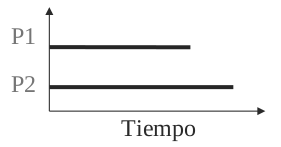
\includegraphics[scale=0.63]{real}
					\caption{Real o paralela}
				\end{figure}
			
				Si el número de procesadores es menor al número de procesos, entonces se da concurrencia aparente o simulada, también llamada pseudoparalelismo.\\
			
				\begin{figure}[H]
					\centering
					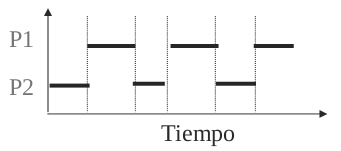
\includegraphics[scale=0.63]{llike}
					\caption{Aparente, simulada o pseudoparalela}
				\end{figure}
				
				\newpage
				
		\subsection{Comunicación entre procesos}
		
			Los procesos de un sistema no actúan de forma aislada.\\
			
			A veces tiene que \underline{cooperar} para alcanzar un objetivo común. A este tipo de comunicación se le llama \textbf{sincronización}.\\
			
			Por contrapartida, a veces tienen que \underline{competir} por el uso de recursos. Esto es lo que se denomina \textbf{exclusión mutua}.\\
			
			\subsubsection{Exclusión mutua}
			
				Los tipos de recursos que existen en exclusión mutua son:\\
			
				- \textbf{Compartibles:} Pueden ser usados por varios procesos de forma concurrente.\\
			
				- \textbf{No compartibles:} Su uso está restringido a un sólo proceso a la vez hasta que el proceso que está usando dicho recurso finaliza su utilización.\\
			
				Es por ello que la exclusión mutua se da cuando dos o más procesos se están ejecutando en paralelo y necesitan a la vez el uso de un recurso no compartible.\\
			
				En este caso, el recurso no compartible se le asigna sólamente a un proceso y el resto queda en espera hasta que el primero finalice de usarlo. Cuando esto ocurra, el recurso será asignado a uno de los procesos en espera. Con ello se asegura \textit{el correcto uso del recurso}.\\
			
				El trozo de código donde un proceso hace uso de un recurso no compartible se denomina \textbf{sección crítica o región crítica} y deben ser ejecutadas lo más rápido posible y cuidadosamente codificadas.\\
				
				\newpage
				
			\subsubsection{Sincronización}
				
				La sincronización es la comunicación requerida entre dos o más procesos con el fin de sincronizar sus actividades.\\
				
				Existen dos tipos de sincronización generales:\\
					
				- \textbf{Sincronización simple:} Un proceso, P1, llegado a cierto punto clave, no puede proseguir con su ejecución, hasta que otro proceso, P2, haya llegado a otro punto clave de ejecución.\\
					
				\begin{figure}[H]
					\centerline{\xymatrix{
						P1 \ar@/_/[dr] & & P1 \\
						P2 \ar[r] & \oslash \ar@/_/[ur] \ar[r] & P2 \\
					}}
				\end{figure}
					
				- \textbf{Sincronización múltiple:} Un proceso, P1, llegado a cierto punto clave de su ejecución no puede proseguir hasta que otro proceso, P2, no haya llegado a dicho punto, y viceversa.\\
					
				\begin{figure}[H]
					\centerline{\xymatrix{
						P1 \ar@/_/[dr] & & P1 \\
						& \oslash \ar@/_/[ur] \ar@/^/[dr]& \\
						P2 \ar@/^/[ur] & & P2 \\
					}}
				\end{figure}
			
				\newpage
					
		\subsection{Interbloqueos o Deadlocks}
		
			Un proceso está \textbf{interbloqueado} si está esperando por un evento determinado que nunca va a ocurrir.\\
		
			Un conjunto de procesos está \textbf{interbloqueado} cuando cada uno de ellos está esperando un suceso que sólo puede ser causado por otro proceso del mismo conjunto y que nunca se producirá porque están bloqueados.\\
		
			\begin{figure}[H]
				\centerline{\xymatrix{
				& \fbox{Recurso~NC~1} \ar@/_/[ld] & \\
				\ovalbox{Proceso~A} \ar@{-->}@/_/[dr] & \bigotimes & \ovalbox{Proceso~B} \ar@{-->}@/_/[ul] \\
				& \fbox{Recurso~NC~2} \ar@/_/[ru] & \\
			}}
				\caption*{Interbloque entre dos procesos por el uso de recursos no compartibles}
			\end{figure}
		
			Un proceso está \textbf{postergado indefinidamente} cuando espera por un evento que puede ocurrir pero no se sabe cuando.\\
		
			Un proceso puede quedar esperando indefinidamente si no puede proseguir su ejecución debido al continuo procesamiento de otro proceso por parte del Sistema Operativo.\\
		
			\subsubsection{Condiciones necesarias para el interbloqueo}
			
				- \textbf{Exclusión mutua:} Los procesos reclaman control excesivo de los recursos que piden.\\
				
				- \textbf{Esperar por:} Los procesos mantienen los recursos que ya les han asignado mientras esperan por recursos adicionales.\\
				
				-\textbf{No apropiatividad:} Los recursos no pueden ser extraídos de los procesos que los mantienen hasta su completa utilización.\\
				
				- \textbf{Espera circular:} Existe una cadena circular de procesos en la cual uno de ellos mantiene uno o más recursos que son requeridos por el siguiente proceso de la cadena.\\
				
			\subsubsection{Prevención del interbloqueo}
			
				Para prevenir el interbloqueo, podemos realizar tres acciones:\\
			
				- \textbf{Negar la condición de \textit{esperar por}:} Cada proceso debe pedir todos los recursos que va a necesitar de golpe. Si el conjunto de todos ellos está disponible, se le asigna todos. En caso contrario, no se le asigna a ningún proceso y tendrá que esperar hasta que todos estén disponibles.\\
				
				- \textbf{Negar la condición de \textit{no apropiatividad}:} Cuando un proceso que tiene recursos le es negada una petición de recursos adicionales, deberá liberar sus recursos y, si es necesario, pedirlos de nuevo junto a los recursos adicionales.\\
				
				- \textbf{Negar la condición de \textit{espera circular}:} Cuando se intala un recurso, se le asigna un número exclusivo, de forma que los procesos deben solicitar los recursos en orden ascendente.\\
				
				Con esto podemos prevenirlo \textbf{evitando} el interbloqueo condicionando al sistema para que esquive determinadas situaciones propensas a ello, \textbf{detectando} y determinando si existe o no dicho interbloqueo identificando qué procesos y recursos están implicados en él o \textbf{recuperarnos} de uno retirando uno o más condiciones necesarias.\\
				
		\newpage
				
		\subsection{Estados de un proceso}
			
			\vfill
			
			\begin{figure}[H]
				\centerline{\xymatrix{
				Se~crea~el~proceso \ar@{-->}@/_/[ddr] & & Se~termina~el~proceso \\
				\\
				asignacion~de~la~CPU & \ovalbox{ ACTIVO } \ar@/^/[dr] \ar@/_/@{-->}[uur] & esperar~evento \\
		\ovalbox{ LISTO } \ar@/^/[ur] & & \ovalbox{ BLOQUEADO } \ar@/^/[ll] \\
				& ocurre~el~evento & \\
				\\
				}}
			\end{figure}	
											
			Un proceso está \textbf{activo} cuando tiene el control de un procesador.\\
			
			Un proceso está \textbf{bloqueado} cuando está esperando a que ocurra un evento.\\
			
			Un proceso está \textbf{listo} cuando está esperando para usar un procesador.\\
			
			\newpage
			
			\subsubsection{Bloque de Control de Procesos (PCB)}
			
				El Bloque de Control de Procesos o PCB es una estructura de datos que contiene toda la información de un proceso que el Sistema Operativo necesita para su control.\\
			
			Guarda 	parámetros de estado volátil, como el estado actual, identificación, punteros a memoria, punteros de recursos, etc.\\
			
		\subsubsection{Bloque de Control del Sistema (SCB)}
		
			El Bloque de Control del Sistema o SCB es una estructura de datos que gestiona el Sistema Operativo para controlar todos los PCB's de los procesos. Reside en memoria principal por su alta frecuencia de consulta.\\
			
			Guarda parámetros como la lista de PCB's, punteros a los PCB's activos, puntero a la lista de procesos listos, puntero a la lista de procesos bloqueados, etc.
		\subsubsection{Operaciones básicas sobre procesos}
		
			- \textbf{Crear un proceso}: dar nombre al proceso, insertarlo en la lista de procesos en estado listo, determinar su prioridad inicial, crear el PCB del proceso y asignarles los recursos iniciales del proceso.\\
			
			- \textbf{Destruir un proceso}: devolver al sistema los recursos que tiene asignado, eliminarlo de todas las listas del sistema y borrar su PCB.\\
			
			- \textbf{Cambiar la prioridad de un proceso}.\\
			
			- \textbf{Bloquear un proceso}.\\
			
			- \textbf{Despertar un proceso}.\\
			
			- \textbf{Despachar un proceso}.\\
			
			\newpage
			
	\section{El núcleo del Sistema Operativo. El kernel}
	
		\vfill
			
		El kernel se ejecuta con las interrupciones desactivadas (\textbf{modo privilegiado}) y es la parte del Sistema Operativo más cercana al hardware, por ello suele estar codificado en ensamblador o en lenguaje máquina y reside en la memoria principal.\\
		
		\subsection{Funciones básicas del kernel}
		
			a) Manipulación de interrupciones.\\
			
			b) Inhabilitación y habilitación de interrupciones.\\
			
			c) Creación y destrucción de procesos.\\
			
			d) Cambio de estado de un proceso.\\
			
			e) Despachar un proceso.\\
			
			f) Comunicación entre procesos.\\
			
			g) Manipulación de los PCB's.\\
			
			h) Soporte para servicios de más alto nivel.\\
			
			\newpage
			
\end{document}